\documentclass[fontset=none]{Notes}

\makeatletter
\DeclareRobustCommand{\em}{%
  \@nomath\em \if b\expandafter\@car\f@series\@nil
  \normalfont \else \bfseries \fi}
\makeatother

\usepackage{tikz-cd,wrapstuff}
\usepackage{siunitx,tikz,nicematrix}
\usetikzlibrary{matrix,calc}
\usetikzlibrary{intersections}
\usetikzlibrary{arrows.meta}

\ProvidesFile{font.def}

\setCJKmainfont{Source Han Serif SC}[
  UprightFont=*-Regular,
  BoldFont=*-Bold,
  ItalicFont=HYKaiTi S,
  ItalicFeatures={Scale=1.1}
]
\newCJKfontfamily[zhsong]\songti{Source Han Serif SC}[
  UprightFont=*-Regular,
  BoldFont=*-Bold,
  ItalicFont=HYKaiTi S,
  ItalicFeatures={Scale=1.1}
]
\setCJKsansfont{Source Han Sans SC}[
  UprightFont=*-Regular,
  BoldFont=*-Bold
]
\newCJKfontfamily[zhhei]\heiti{Source Han Sans SC}[
  UprightFont=*-Regular,
  BoldFont=*-Bold
]
\setCJKmonofont{HYFangSong S}[
  BoldFont=*,
  ItalicFont=*,
  BoldItalicFont=*
]
\newCJKfontfamily[zhfs]\fangsong{HYFangSong S}[
  BoldFont=*,
  ItalicFont=*,
  BoldItalicFont=*
]
\newCJKfontfamily[zhkai]\kaishu{HYKaiTi S}[
  BoldFont=*,
  ItalicFont=*,
  BoldItalicFont=*
]

\setmainfont{texgyretermes}[
  Extension=.otf,
  UprightFont=*-regular,
  BoldFont=*-bold,
  ItalicFont=*-italic,
  BoldItalicFont=*-bolditalic,
  SlantedFont=*-italic
]
%\setmathrm{texgyretermes}[
%  Extension=.otf,
%  UprightFont=*-regular,
%  BoldFont=*-bold,
%  ItalicFont=*-italic,
%  BoldItalicFont=*-bolditalic,
%  SlantedFont=*-italic
%]
\setsansfont{Cantarell}[
  UprightFont=* Regular,
  ItalicFont=* Italic,
  BoldFont=* Bold,
  BoldItalicFont=* Bold Italic,
  SmallCapsFont=Alegreya Sans SC
]
\setmonofont{Ubuntu Mono}[
  UprightFont=*,
  ItalicFont=* Italic,
  BoldFont=* Bold,
  BoldItalicFont=* Bold Italic
]
%\setmathfont{texgyretermes-math.otf}
%\setmathfont[range={\mathcal,\mathbfcal,\mathfrak},StylisticSet=1]{XITSMath-Regular.otf}
%\setmathfont[range={\mathbb}]{KpMath-Sans.otf}



\usepackage[subscriptcorrection,nofontinfo,mtpbb,mtpfrak]{mtpro2}
\usepackage[normal]{fixdif}

\tikzcdset{
  arrow style=tikz,
  diagrams={>={Straight Barb[scale=0.8]}}
}

\tikzset{
  every picture/.style={
    thick,
    >={Latex[width=6pt, length=8pt]}
  },
  point/.style={
    circle, fill, minimum width=5pt,
    inner sep=0pt
  }
}

\allowdisplaybreaks[1]

\newlength{\mymathln}
\newcommand{\aligninside}[2]{
  \settowidth{\mymathln}{#2}
  \mathmakebox[\mymathln]{#1}
}

\DeclareMathOperator\Spec{Spec}
\DeclareMathOperator\im{im}
\DeclareMathOperator\sgn{sgn}
\DeclareMathOperator\rad{rad}
\DeclareMathOperator\Alt{Alt}
\DeclareMathOperator\Max{Max}
\DeclareMathOperator\GL{GL}
\DeclareMathOperator\Orth{O}
\DeclareMathOperator\SO{SO}
\DeclareMathOperator\SU{SU}
\DeclareMathOperator\Lie{Lie}
\DeclareMathOperator\End{End}
\DeclareMathOperator\Int{Int}
\DeclareMathOperator\Sym{Sym}
\DeclareMathOperator\tr{tr}
\DeclareMathOperator\Hom{Hom}
\DeclareMathOperator\supp{supp}
\DeclareMathOperator\Id{Id}
\DeclareMathOperator\rk{rank}
\DeclareMathOperator\grad{grad}
\DeclareMathOperator\Euc{E}
\DeclareMathOperator\ob{ob}
\newcommand{\LL}{{\mathrm{L}}}

\newcommand{\ideal}[1]{\mathfrak{#1}}
\newcommand{\mat}[1]{\mathbold{#1}}
\newcommand{\cat}[1]{\mathsf{#1}}
\newcommand{\uline}{\underline{\hphantom{X}}}
\newcommand{\abs}[1]{\left|#1\right|}
\newcommand{\lie}[1]{\mathfrak{#1}}
\newcommand{\inn}[1]{\left\langle #1\right\rangle}

\usepackage{enumitem}

\setlist[enumerate]{nosep}

%\DeclareMathAlphabet\mathcal{OMS}{cmsy}{m}{n}

\newlength\stextwidth
\newcommand\makesamewidth[3][c]{%
  \settowidth{\stextwidth}{#2}%
  \makebox[\stextwidth][#1]{#3}%
}



\begin{document}

\frontmatter

\tableofcontents

\mainmatter

\setcounter{chapter}{-1}

\chapter{导论}

\section{Brouwer 不动点定理}

我们首先概述 Brouwer 不动点定理的证明:如果 $f:D^n\to D^n$ 是连续映射,
那么存在 $x\in D^n$ 使得 $f(x)=x$。当 $n=1$ 的时候,这个定理是容易证明的,
此时 $D^1$ 是闭区间 $[-1,1]$,我们在正方形 $D^1\times D^1$ 内观察
$f$ 的图像。
\begin{figure}[h]
  \centering
  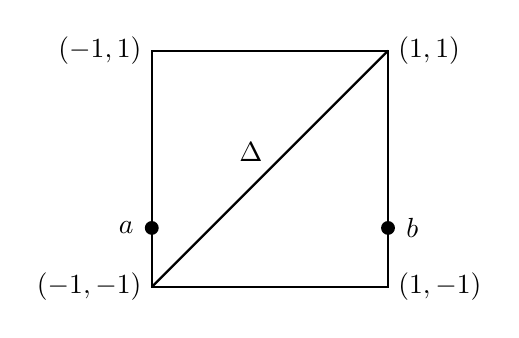
\begin{tikzpicture}[
      scale=1.5
    ]
    \draw (-1,-1) coordinate (v1) rectangle (1,1) coordinate (v2);
    \draw (v1) -- node[midway,above left=-1pt] {$\Delta$} (v2);
    \node [point,label=180:$a$] at ([yshift=0.5cm]v1) {};
    \node [point,label=0:$b$] at ([yshift=0.5cm]v1-|v2) {};
    \node [left] at (v1) {$(-1,-1)$};
    \node [left] at (v1|-v2) {$(-1,1)$};
    \node [right] at (v2) {$(1,1)$};
    \node [right] at (v2|-v1) {$(1,-1)$};
  \end{tikzpicture}
\end{figure}

\begin{theorem}
  每个连续映射 $f:D^1\to D^1$ 都有一个不动点。
\end{theorem}
\begin{proof}
  设 $f(-1)=a$ 以及 $f(1)=b$。要是 $f(-1)=-1$ 或者 $f(1)=1$,那么
  这就已经存在不动点,所以我们假设 $f(-1)=a>-1$ 以及 $f(1)=b<1$。
  设 $G$ 是 $f$ 的图像,$\Delta$ 是恒等映射的图像(对角线),我们需要证明
  $G\cap\Delta\neq \emptyset$。想法是利用连通性说明 $D^1\times D^1$
  中从 $a$ 到 $b$ 的道路必须与 $\Delta$ 相交。$f$ 连续表明 
  $G=\{(x,f(x))\,|\, x\in D^1\}$ 是连通的。定义 $A=\{(x,f(x))\,|\, f(x)>x\}$
  和 $B=\{(x,f(x))\,|\, f(x)<x\}$,注意到 $a\in A$ 和 $b\in B$。
  假设 $G\cap \Delta=\emptyset$,那么这表明 $G=A\cup B$ 是无交并,而
  $A,B$ 都是 $G$ 中的非空开集,与 $G$ 连通矛盾。
\end{proof}

不幸的是,当 $n>1$ 的时候没有人知道如何应用这个初等的拓扑证明,所以
必须引入新的思想。通过代数拓扑可以给出 Brouwer 不动点定理的一个证明。
我们最终将证明,对于每个 $n\geq 0$,存在一个\emph{同调函子} $H_n$
使得:对于每个拓扑空间 $X$,都给出一个交换群 $H_n(X)$;
对于每个连续映射 $f:X\to Y$,都给出一个同态 $H_n(f):H_n(X)\to H_n(Y)$
使得
\begin{equation}
  H_n(g\circ f)=H_n(g)\circ H_n(f)
\end{equation}
以及 $H_n(1_X)$ 是 $H_n(X)$ 上的恒等映射;此外还有
\begin{alignat}{2}
  &H_n(D^{n+1})=0 &\quad &\text{for all $n\geq 1$},\\
  &H_n(\mathbb{S}^{n})\neq 0 &&\text{for all $n\geq 1$}
  \label{eq:H_n(S^n)}.
\end{alignat}
使用 $H_n$ 的这些性质,我们现在可以证明 Brouwer 不动点定理。

\begin{definition}
  拓扑空间 $Y$ 的一个子空间 $X$ 被称为 $Y$ 的一个\emph{收缩},如果
  存在连续映射 $r:Y\to X$ 使得对于所有的 $x\in X$ 有 $r(x)=x$。
  这样的 $r$ 被称为一个\emph{收缩映射}。
\end{definition}

\begin{remark}
  (1)
  我们可以使用映射的语言重新叙述收缩映射的定义。如果 $\iota:X\hookrightarrow Y$
  是包含映射,那么连续映射 $r:Y\to X$ 是收缩映射当且仅当 $\iota$ 是 $r$ 的右逆,
  即 $r\circ\iota=1_X$。

  (2) 对于交换群来说,可以证明 $G$ 的子群 $H$ 是 $G$ 的收缩当且仅当 
  $H$ 是 $G$ 的一个直和项,也即存在 $G$ 的子群 $K$ 使得 $G=H\oplus K$。
\end{remark}

\begin{lemma}\label{lemma:S^n is not retract of D^n+1}
  如果 $n\geq 0$,那么 $\mathbb{S}^n$ 不是 $D^{n+1}$ 的收缩。
\end{lemma}
\begin{proof}
  假设存在收缩 $r:D^{n+1}\to \mathbb{S}^n$,那么我们有交换图
  \[
    \begin{tikzcd}[column sep=1.8em]
      & D^{n+1}\arrow[dr,"r"] & \\
      \mathbb{S}^n\arrow[ur,"\iota"]\arrow[rr,"1"'] & & \mathbb{S}^n ,
    \end{tikzcd}
  \]
  利用函子 $H_n$,给出了交换群的一个交换图
  \[
    \begin{tikzcd}[column sep=1em]
      & H_n(D^{n+1})\arrow[dr,"H_n(r)"] & \\
      H_n(\mathbb{S}^n)\arrow[ur,"H_n(\iota)"]\arrow[rr,"H_n(1)"'] & & 
      H_n(\mathbb{S}^n ),
    \end{tikzcd}
  \]
  由于 $H_n(D^{n+1})=0$,所以 $H_n(1)=H_n(\iota)\circ H_n(r)=0$,但是
  $H_n(1)$ 又必须是恒等映射,所以 $H_n(\mathbb{S}^n)=0$,这
  和 \eqref{eq:H_n(S^n)} 矛盾。
\end{proof}

注意到同调函子 $H_n$ 将拓扑问题转化为了代数问题。此外,
\autoref{lemma:S^n is not retract of D^n+1} 在 $n=0$ 的时候有很简单的证明,
此时收缩 $r:D^1\to \mathbb{S}^0=\{\pm 1\}$ 将连通空间映射到不连通空间,
这是不可能的。

\begin{theorem}[Brouwer]\label{thm:Brouwer}
  如果 $f:D^n\to D^n$ 是连续映射,那么 $f$ 有一个不动点。
\end{theorem}
\begin{proof}
  假设对于所有的 $x\in D^n$ 都有 $f(x)\neq x$,此时 $x$ 和 $f(x)$
  确定了一条直线。定义 $g:D^n\to \mathbb{S}^{n-1}$ 将 $x$ 映射
  为 $f(x)$ 到 $x$ 的射线与 $\mathbb{S}^{n-1}$ 的交点。
  \begin{center}
    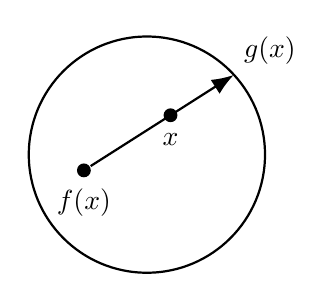
\begin{tikzpicture}
      \draw [name path=circ] (0,0) circle (1.5);
      \node [point,label=-90:$x$] (x) at (0.3,0.5) {}; 
      \node [point,label=-90:$f(x)$] (fx) at (-0.8,-0.2) {};
      \path [name path=line] (fx) -- ($(fx)!2!(x)$);
      \draw [->,name intersections={of=circ and line, by={gx}}]
        (fx) -- (gx) node [above right] {$g(x)$};
    \end{tikzpicture}
  \end{center}
  显然
  $x\in \mathbb{S}^{n-1}$ 表明 $g(x)=x$。利用坐标不难计算得 $g$ 
  是连续映射。
  这样 $g$ 就构成了一个收缩映射,与前面的引理矛盾。
\end{proof}

\begin{problem}{}{}
令 $H$ 是交换群 $G$ 的子群。如果存在同态 $r:G\to H$ 使得
对任意 $x\in H$ 有 $r(x)=x$,那么 $G=H\oplus \ker r$。  
\end{problem}
\begin{proof}
  任取 $y\in G$,那么 $r(y-r(y))=r(y)-r(y)=0$,所以
  $y-r(y)\in\ker r$,所以 $y=r(y)+y-r(y)\in H+\ker r$,
  所以 $G=H+\ker r$。下面设 $x\in H\cap\ker r$,那么
  $x=r(x)=0$,所以 $H\cap\ker r=\emptyset$。
\end{proof}

\begin{problem}{}{}
  假设在 $n\geq 1$ 的时候已知
  \[
    H_i(\mathbb{S}^n)=\begin{cases}
      \mathbb{Z} & i=0,n,\\
      0 & \text{otherwise},
    \end{cases}
  \]
  证明 $\mathbb{S}^{n}$ 的赤道不是一个收缩。
\end{problem}
\begin{proof}
  设 $r:\mathbb{S}^n\to \mathbb{S}^{n-1}$ 是收缩映射。
  那么我们有交换图
  \[
    \begin{tikzcd}[column sep=1em]
      & H_i(\mathbb{S}^{n})\arrow[dr,"H_i(r)"] & \\
      H_i(\mathbb{S}^{n-1})\arrow[ur,"H_i(\iota)"]\arrow[rr,"H_i(1)"'] & & 
      H_i(\mathbb{S}^{n-1}),
    \end{tikzcd}
  \]
  取 $i=n-1$ 即可得出矛盾。
\end{proof}

\begin{problem}{}{}
  如果 $X$ 是同胚于 $D^n$ 的拓扑空间,那么连续映射
  $f:X\to X$ 有不动点。
\end{problem} 
\begin{proof}
  设 $\varphi:D^n\to X$ 是同胚映射,那么 $\varphi^{-1}\circ f\circ\varphi:D^n\to D^n$
  是连续映射且有不动点,即存在 $x$ 使得 $\varphi^{-1}(f(\varphi(x)))=x$,
  即 $f(\varphi(x))=\varphi(x)$,所以 $f$ 有不动点 $\varphi(x)$。
\end{proof}

\begin{problem}{}{}
  令 $f,g:I\to I\times I$ 是连续映射,并且 $f(0)=(a,0)$,
  $f(1)=(b,1)$,$g(0)=(0,c)$,$g(1)=(1,d)$。证明存在 $s,t\in I$
  使得 $f(s)=g(t)$,也就是说 $f$ 和 $g$ 的像集一定是相交的道路。
\end{problem}
\begin{proof}
  定义 $h:I\times I\to I\times I$ 为
\end{proof}


\section{范畴与函子}

\begin{definition}
  范畴 $\cat C$ 上的一个\emph{共轭}指的是所有态射的类 $\bigcup_{(A,B)}\Hom(A,B)$
  上的一个等价关系 $\sim$,满足:
  \begin{enumerate}
    \item 如果 $f\in\Hom(A,B)$ 以及 $f\sim f'$,那么 $f'\in\Hom(A,B)$;
    \item 如果 $f\sim f'$ 和 $g\sim g'$ 并且 $g\circ f$ 存在,那么
    $g\circ f\sim g'\circ f'$。
  \end{enumerate}
\end{definition}

\begin{theorem}
  令 $\cat C$ 是一个范畴附带一个共轭 $\sim$,令 $[f]$ 表示态射 $f$ 的等价类。
  定义 $\cat C'$ 为:
  \begin{align*}
    \ob \cat C'&=\ob \cat C;\\
    \Hom_{\cat C'}(A,B)&=\bigl\{[f]\bigm| f\in\Hom_{\cat C}(A,B)\bigr\};\\
    [g]\circ [f]&=[g\circ f].
  \end{align*}
  那么 $\cat C'$ 是一个范畴,称为 $\cat C'$ 的\emph{商范畴}。
\end{theorem}

\chapter{基本拓扑概念}

\section{同伦}

\begin{definition}
  如果 $X,Y$ 是拓扑空间,$f_0,f_1$ 是 $X$ 到 $Y$ 的连续映射,存在
  连续映射 $F:X\times I\to Y$ 使得
  \[
    F(x,0)=f_0(x),\quad F(x,1)=f_1(x),
  \]
  那么我们说 $F$ 是一个\emph{同伦映射},并且 $f_0$ \emph{同伦于}
  $f_1$,记为 $f_0\simeq f_1$。当需要强调同伦映射的时候,我们写作
  $F:f_0\simeq f_1$。
\end{definition}

如果记 $f_t:X\to Y$ 为 $f_t(s)=F(x,t)$,那么同伦 $F$ 给出了一族
从 $f_0$ 变形到 $f_1$ 的单参数连续映射。我们可以认为 $f_t$ 随着
时间 $t$ 变形。

\begin{lemma}[粘连引理]
  假设 $X$ 是有限个闭子集的并集:$X=\bigcup_{i=1}^n X_i$。
  如果对于某个空间 $Y$,存在一族连续映射 $f_i:X_i\to Y$,它们在
  重叠区域相同,即对于任意 $i,j$ 有 $f_i|_{X_i\cap X_j}=f_j|_{X_i\cap X_j}$,
  那么存在唯一的连续映射 $f:X\to Y$ 使得对于所有的 $i$ 有 $f|_{X_i}=f_i$。
\end{lemma}
\begin{proof}
  任取 $x\in X$,如果 $x\in X_i$,我们定义 $f(x)=f_i(x)$。
  由于 $f_i,f_j$ 在重叠区域相同,所以这个定义是良好的,我们只需要说明连续性。
  任取 $Y$ 的闭子集 $C$,那么
  \begin{equation*}
    f^{-1}(C)=\bigcup\bigl(X_i\cap f^{-1}(C)\bigr)=
    \bigcup f_i^{-1}(C),
  \end{equation*}
  由于 $f_i^{-1}(C)$ 是 $X_i$ 的闭集,所以是 $X$ 的闭集。
  所以 $f^{-1}(C)$ 是闭集,即 $f$ 是连续映射。
\end{proof}

粘合引理也可以有开集的版本,其证明是完全一致的。

\begin{lemma}{}{}
  假设 $X$ 是任意个开子集的并集:$X=\bigcup_i X_i$。
  如果对于某个空间 $Y$,存在一族连续映射 $f_i:X_i\to Y$,它们在
  重叠区域相同,
  那么存在唯一的连续映射 $f:X\to Y$ 使得对于所有的 $i$ 有 $f|_{X_i}=f_i$。
\end{lemma}

\begin{theorem}
  同伦是所有连续映射 $X\to Y$ 集合上的一个等价关系。
\end{theorem}
\begin{proof}
  \emph{自反性}。如果 $f:X\to Y$ 是连续映射,定义 $F(x,t)=f(x)$,
  显然 $F:f\simeq f$。

  \emph{对称性}。假设 $f\simeq g$,即存在连续映射 $F:X\times I\to Y$
  使得 $F(x,0)=f(x)$ 和 $F(x,1)=g(x)$。定义 $G:X\times I\to Y$
  为 $G(x,t)=F(x,1-t)$,那么 $G:g\simeq f$。

  \emph{传递性}。假设 $F:f\simeq g$ 以及 $G:g\simeq h$。定义
  $H:X\times I\to Y$ 为
  \[
    H(x,t)=\begin{cases}
      F(x,2t) & 0\leq t\leq \frac{1}{2},\\
      G(x,2t-1) & \frac{1}{2}\leq t\leq 1.
    \end{cases}
  \]
  根据粘合引理,所以 $H$ 连续,所以 $H:f\simeq h$。
\end{proof}

\begin{definition}
  如果 $f:X\to Y$ 是连续映射,我们说
  \[
    [f]=\{g:X\to Y\,|\, g\simeq f\}
  \]
  是 $f$ 的\emph{同伦类}。
\end{definition}

所有同伦类的集合记为 $[X,Y]$。

\begin{theorem}
  对于 $i=0,1$,令 $f_i:X\to Y$ 和 $g_i:Y\to Z$ 是连续映射。如果
  $f_0\simeq f_1$ 和 $g_0\simeq g_1$,那么 $g_0\circ f_0\simeq g_1\circ f_1$,
  即 $[g_0\circ f_0]=[g_1\circ f_1]$。
\end{theorem}
\begin{proof}
  令 $F:f_0\simeq f_1$ 和 $G:g_0\simeq g_1$ 是同伦映射。
  首先定义 $H:X\times I\to Z$ 为 $H(x,t)=G(f_0(x),t)$,
  那么 $H:g_0\circ f_0\simeq g_1\circ f_0$。
  另一方面,定义 $K:X\times I\to Z$ 为 $K(x,t)=g_1\circ F(x,t)$,
  那么 $K:g_1\circ f_0\simeq g_1\circ f_1$。
  根据同伦的传递性,就有 $g_1\circ f_1\simeq g_0\circ f_0$。
\end{proof}

\begin{corollary}
  同伦是拓扑范畴 $\cat{Top}$ 上的一个共轭。
\end{corollary}

这意味着存在一个商范畴,其对象是拓扑空间 $X$,态射集合 
$\Hom(X,Y)=[X,Y]$,复合为 $[g]\circ [f]=[g\circ f]$。

\begin{definition}
  上述商范畴被称为\emph{同伦范畴},记为 $\cat{hTop}$。
\end{definition}

我们即将构造的所有从 $\cat{Top}$ 到某个“代数”范畴 $\cat A$(例如 $\cat{Ab},\cat{Grp},\cat{Ring}$)
的函子 $T:\cat{Top}\to\cat{A}$ 都有性质使得 $f\simeq g$ 的时候有 $T(f)=T(g)$。
事实上,除开自然地希望将同伦映射视为等同的之外,这保证了通过 $T$
将拓扑问题转化为 $\cat A$ 中的代数问题是比原问题更加简单的。
此外,练习表明每个这样的函子都会给出一个函子 $\cat{hTop}\to\cat A$,
所以同伦范畴是相当基本的。

\begin{definition}
  一个连续映射 $f:X\to Y$ 被称为\emph{同伦等价},如果存在连续映射
  $g:Y\to X$ 使得 $g\circ f\simeq 1_X$ 和 $f\circ g\simeq 1_Y$。
  如果存在同伦等价 $f:X\to Y$,那么我们说空间 $X$ 和 $Y$
  有相同的\emph{同伦型}。
\end{definition}

显然,同胚的空间有相同的同伦型,但是反过来不对,我们将在后面看到。

下面的两个结果表明同伦可以和一些有趣的问题联系起来。

\begin{definition}
  令 $X,Y$ 是拓扑空间,$y_0\in Y$。$y_0$ 处的\emph{常值映射}
  指的是映射 $c:X\to Y$ 使得 $c(x)\equiv y_0$。
  对于连续映射 $f:X\to Y$,如果存在常值映射 $c$ 使得 $f\simeq c$,那么我们说 $f$ 是
  \emph{零伦的}。
\end{definition}

\begin{remark}
  我们将在后面看到 $\mathbb{C}\smallsetminus\{0\}$ 实质上是圆周
  $\mathbb{S}^1$,即 $\mathbb{C}\smallsetminus\{0\}$ 和 $\mathbb{S}^1$
  有相同的同伦型。
\end{remark}





\end{document}
